\documentclass[border=10pt,varwidth]{standalone}
\usepackage[left=25mm,right=25mm,top=25mm,bottom=25mm]{geometry}
\usepackage[utf8]{inputenc}
\usepackage[T1]{fontenc}
\usepackage{times}
\usepackage{geometry}
\usepackage{amsmath}
\usepackage{amssymb}
\usepackage{mathrsfs}
\usepackage{amsfonts}
\usepackage{amsthm}
\usepackage{lipsum}
\usepackage{amscd}
\usepackage{graphicx}
\usepackage{fancyhdr}
\usepackage{textcomp}
\usepackage{pgfplots}
\usepackage{txfonts}
\usepackage[all]{xy}
\usepackage{paralist}
\usepackage[colorlinks=true]{hyperref}
\usepackage{array}
\usepackage{tikz}
\usepackage{slashed}
\usepackage{pdfpages}
\usepackage{cite}
\usepackage{url}
\usepackage{amsmath,amsfonts,amssymb}
\usepackage{tikz}
\usetikzlibrary{arrows,matrix,positioning}
\usetikzlibrary{overlay-beamer-styles}
\usetikzlibrary{matrix.skeleton}
\usetikzlibrary{automata,positioning}
\usetikzlibrary{decorations.text}
\usepackage{listings}
\usepackage{multirow}
\usepackage{color}

\begin{document}

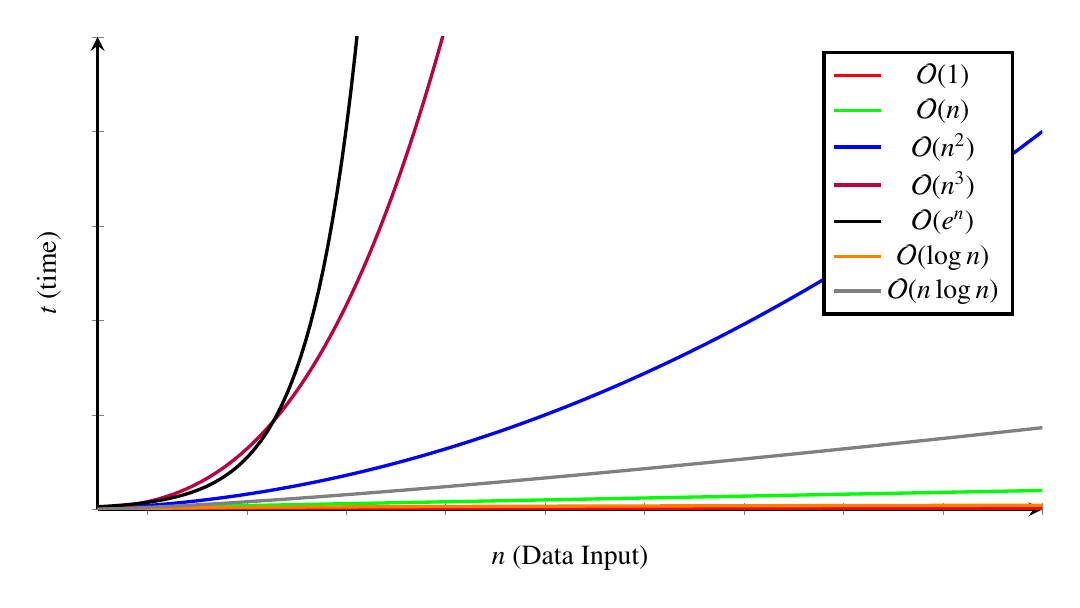
\begin{tikzpicture}
\begin{axis}[
    axis lines = left,
    xlabel = $n$ (Data Input),
    ylabel = {$t$ (time)},
    legend pos=north east,
    very thick,
    ymax = 500,
    yticklabels=\empty,
    xticklabels=\empty,
    scale only axis=true,
  width=12cm, height=6cm,
    ]
\addplot [
    domain= 1:20,
    samples=100,
    color=red,
]
{1};
\addlegendentry{$\mathcal{O}(1)$}
\addplot [
    domain= 1:20,
    samples=100,
    color=green,
]
{x};
\addlegendentry{$\mathcal{O}(n)$}
\addplot [
    domain= 1:20,
    samples=100,
    color=blue,
]
{x^2};
\addlegendentry{$\mathcal{O}(n^2)$}
\addplot [
    domain= 1:10,
    samples=100,
    color=purple,
]
{x^3};
\addlegendentry{$\mathcal{O}(n^3)$}
\addplot [
    domain= 1:10,
    samples=100,
    color=black,
]
{exp(x)};
\addlegendentry{$\mathcal{O}(e^n)$}
\addplot [
    domain= 1:20,
    samples=100,
    color=orange,
]
{log2(x)};
\addlegendentry{$\mathcal{O}(\log n)$}

\addplot [
    domain= 1:20,
    samples=100,
    color=gray,
]
{x*log2(x)};
\addlegendentry{$\mathcal{O}(n \log n)$}
\end{axis}
\end{tikzpicture}

\end{document}
